\documentclass[xcolor=dvipsnames]{beamer}
\usepackage[T1]{fontenc}
\usepackage[utf8]{inputenc}
\usepackage[english,slovak]{babel}

\usepackage{amsmath}
\usepackage{amsthm}
\usetheme{Pittsburgh}
\useoutertheme{shadow}

\usepackage{graphicx}
\usepackage{caption}
\usepackage{subcaption}


\usepackage{listings}
 \setbeamercovered{transparent}
\usepackage{listings}
\lstset{language = C++}







\definecolor{lbcolor}{rgb}{0.9,0.9,0.9}

\lstset{
    % backgroundcolor=\color{lbcolor},
    tabsize=2,
  language=C++,
  captionpos=b,
  tabsize=2,
  frame=lines,
  numbers=left,
  numberstyle=\color{red},
  numberstyle=\tiny,
  numbersep=5pt,
  breaklines=true,
  showstringspaces=false,
  basicstyle=\tiny,
%  identifierstyle=\color{magenta},
  keywordstyle=\color{Fuchsia},
  commentstyle=\color{Gray},
  stringstyle=\color{ForestGreen},
  literate={0}{{\textcolor{BurntOrange}{0}}}{1}%
         {1}{{\textcolor{BurntOrange}{1}}}{1}%
         {2}{{\textcolor{BurntOrange}{2}}}{1}%
         {3}{{\textcolor{BurntOrange}{3}}}{1}%
         {4}{{\textcolor{BurntOrange}{4}}}{1}%
         {5}{{\textcolor{BurntOrange}{5}}}{1}%
         {6}{{\textcolor{BurntOrange}{6}}}{1}%
         {7}{{\textcolor{BurntOrange}{7}}}{1}%
         {8}{{\textcolor{BurntOrange}{8}}}{1}%
         {9}{{\textcolor{BurntOrange}{9}}}{1}%
         {.0}{{\textcolor{BurntOrange}{.0}}}{2}% Following is to ensure that only periods
         {.1}{{\textcolor{BurntOrange}{.1}}}{2}% followed by a digit are changed.
         {.2}{{\textcolor{BurntOrange}{.2}}}{2}%
         {.3}{{\textcolor{BurntOrange}{.3}}}{2}%
         {.4}{{\textcolor{BurntOrange}{.4}}}{2}%
         {.5}{{\textcolor{BurntOrange}{.5}}}{2}%
         {.6}{{\textcolor{BurntOrange}{.6}}}{2}%
         {.7}{{\textcolor{BurntOrange}{.7}}}{2}%
         {.8}{{\textcolor{BurntOrange}{.8}}}{2}%
         {.9}{{\textcolor{BurntOrange}{.9}}}{2}%
  }



%-------------------------------------------------------------------------------------
\title{\bf Stabilizácia robota pomocou gyroskopu}
\author{Michal CHOVANEC}

\date[EURP]{\it September 2017}
\begin{document}

\begin{frame}
\titlepage
\end{frame}



\begin{frame}{\bf Cieľ}

  Naučiť študentov minimálne základy riadania v reálnom čas (odozva jednotky ms) v C++.\\
  Robot bude stabilizovaný pomocou gyroskopu, bude schopný ísť rovno a bude kompenzovať
  pôsobiace bočné sily.

    \begin{itemize}
      \item Modul gyroskopu
      \item Základné triedy a UML
      \item Implementácia v C++ pomocou funktorov
    \end{itemize}

\end{frame}


\begin{frame}{\bf Modul gyroskopu}


\begin{columns}

  \begin{column}{0.5\textwidth}

      \begin{figure}[ht]
      \begin{center}
      \begin{minipage}{0.8\linewidth}
      \begin{center}
      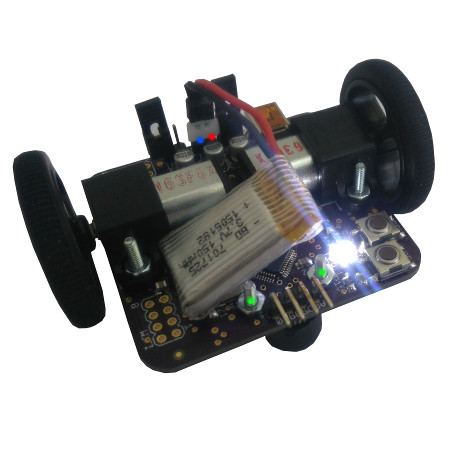
\includegraphics[width=1.0\textwidth]{gyro_module.jpg}
      \end{center}
      \end{minipage}
      \end{center}
      \end{figure}

  \end{column}


  \begin{column}{0.5\textwidth}

  \begin{itemize}
    \item gyroskop LSM6DS0, i2c, 6DOF
    \item Zvolená konfigurácia
          \begin{align*}
            T_s &= 10ms \quad (1ms) \\
            scale &= 500^{\circ}/s \quad (2000^{\circ}/s) \\
            resolution &= 17.50 m^{\circ} / bit \quad (8.75 m^{\circ} / bit)
          \end{align*}

  \end{itemize}

  \end{column}
\end{columns}


\end{frame}



\begin{frame}{\bf UML diagram}



      \begin{figure}[ht]
      \begin{center}
      \begin{minipage}{0.8\linewidth}
      \begin{center}
      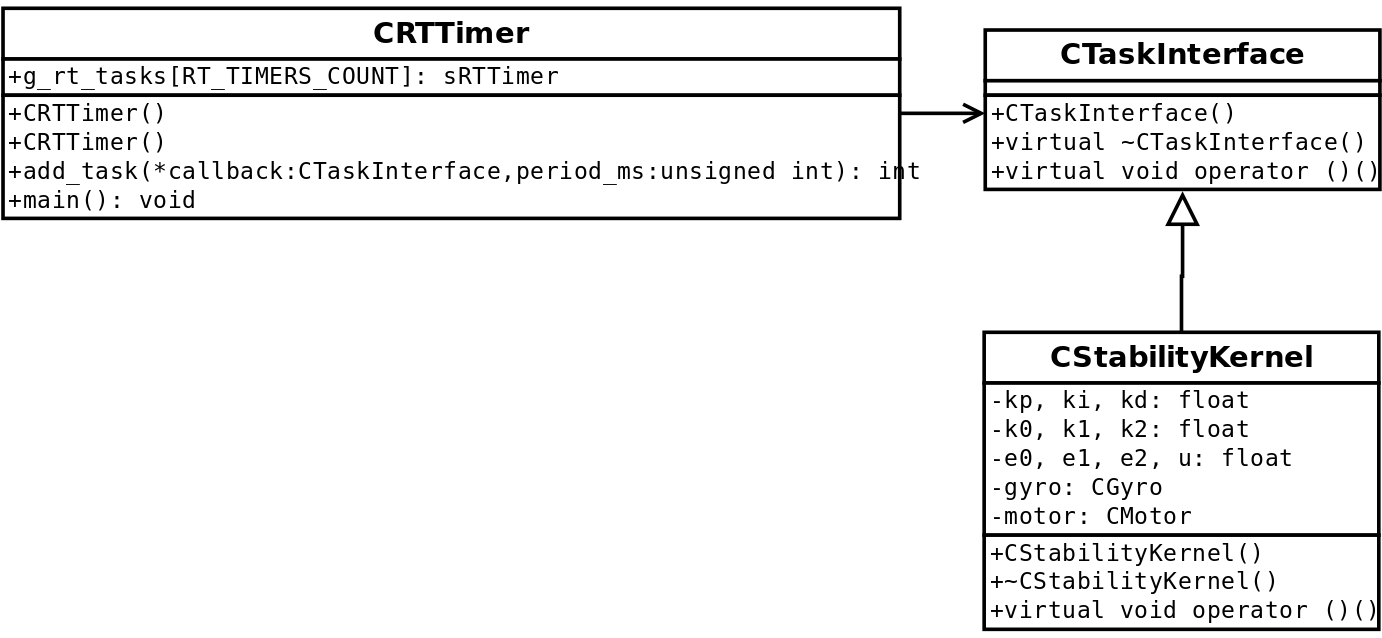
\includegraphics[width=1.0\textwidth]{robot_pid_gyro.png}
      \end{center}
      \end{minipage}
      \end{center}
      \end{figure}



  \begin{itemize}
    \item {\bf CRTTimer} : trieda pre spúštanie úloh v reálnom čase
    \item {\bf CTaskInterface} : virtuálna trieda, predok pre všetky úlohy bežiace v CRTTimer
    \item {\bf CStabilityKernel} : potomok CTaskInterface, obsahuje hlavný riadiaci blok na stabilizáciu robota
  \end{itemize}



\end{frame}

\begin{frame}{\bf Diskrétny tvar PID}
  \begin{align*}
    u(n) &= u(n-1) + k_0e(n) +  k_1e(n-1) +  k_2e(n-2) \\
    k_0 &= k_p + k_i + k_d \\
    k_1 &= -k_p     - 2k_d \\
    k_2 &=         k_d
  \end{align*}

  \begin{itemize}
    \item Ľahko sa implementuje programovo
    \item Odpadajú ''Arduino PID'' problémy napr : \\ $err\_sum+= e(n)$, $dif = e(n) - e(n-1)$
    \item Jednoduchý antiwindup : obmedzenie rozsahu u(n)
    \item Konštanty $k_p, k_i, k_d$ určené experimentálne, pre túto sústavu pochopiteľne $k_i = 0$
  \end{itemize}
\end{frame}


\begin{frame}[fragile]{\bf Implementácia v C++}
    \begin{lstlisting}
    void CStabilityKernel::operator()()
    {
        float speed = 0; //change for forward motion

        gyro.read();

        float angle = 0.0;

        //transform axis (resolution and orientation),
        //for nice PID constants
        angle = -gyro.angles.y*0.1;

        e2 = e1;
        e1 = e0;
        //subtract required and meassured value
        e0 = 0.0 - angle;

        //process PID controller
        u+= k0*e0 + k1*e1 + k2*e2;

        //output for motors, limit output values
        int left  = saturate(u + speed, -256, 256);
        int right = saturate(-u + speed, -256, 256);

        motor.run(left, right);
    }
    \end{lstlisting}
\end{frame}


%-------------------------------------------------------------------------------------
\begin{frame}{\bf Ďakujem za pozornosť}

\url {https://github.com/michalnand/y_robot_course}
\centerline{michal.nand@gmail.com}

\end{frame}

\end{document}
